\subsubsection{06.12.14}

\begin{enumerate}
	\item The time of beginning and ending of the meeting:
	16:10 - 20:10
	\item Purposes of the meeting:
	\begin{enumerate}
	  \item To draw the design for the new bucket.
	  
	  \item To choose the material for the new bucket.
	  
    \end{enumerate}
	\item Work that has been done:
	\begin{enumerate}
	  \item Drew the new design of bucket.
	  
	  \begin{figure}[H]
	  	\begin{minipage}[h]{0.2\linewidth}
	  		\center  
	  	\end{minipage}
	  	\begin{minipage}[h]{0.6\linewidth}
	  		\center{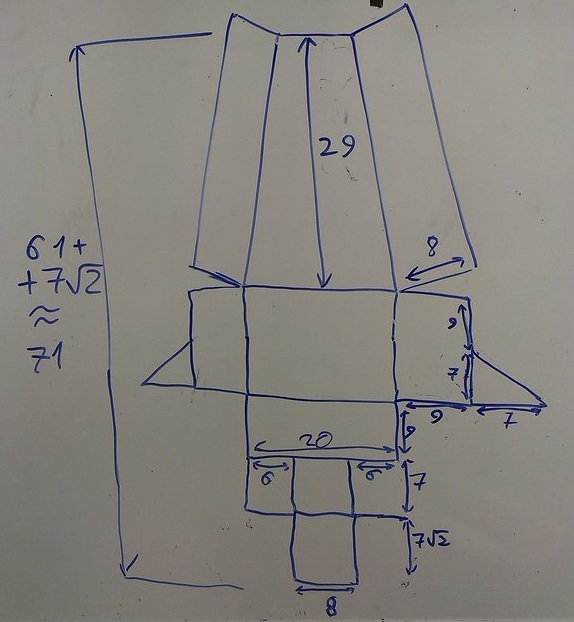
\includegraphics[scale=0.3]{days/06.12.14/images/01}}
	  		\caption{Drawing of projection of bucket with sizes in cm}
	  	\end{minipage}
	  \end{figure}
	  
	  \item For creation of bucket it was decided use PET (type of plastic).
	  
	  \item It turned out that MEL was loose. A transeverse rib of rigidity was added to correct that.
	  
	  \begin{figure}[H]
	  	\begin{minipage}[h]{0.2\linewidth}
	  		\center  
	  	\end{minipage}
	  	\begin{minipage}[h]{0.6\linewidth}
	  		\center{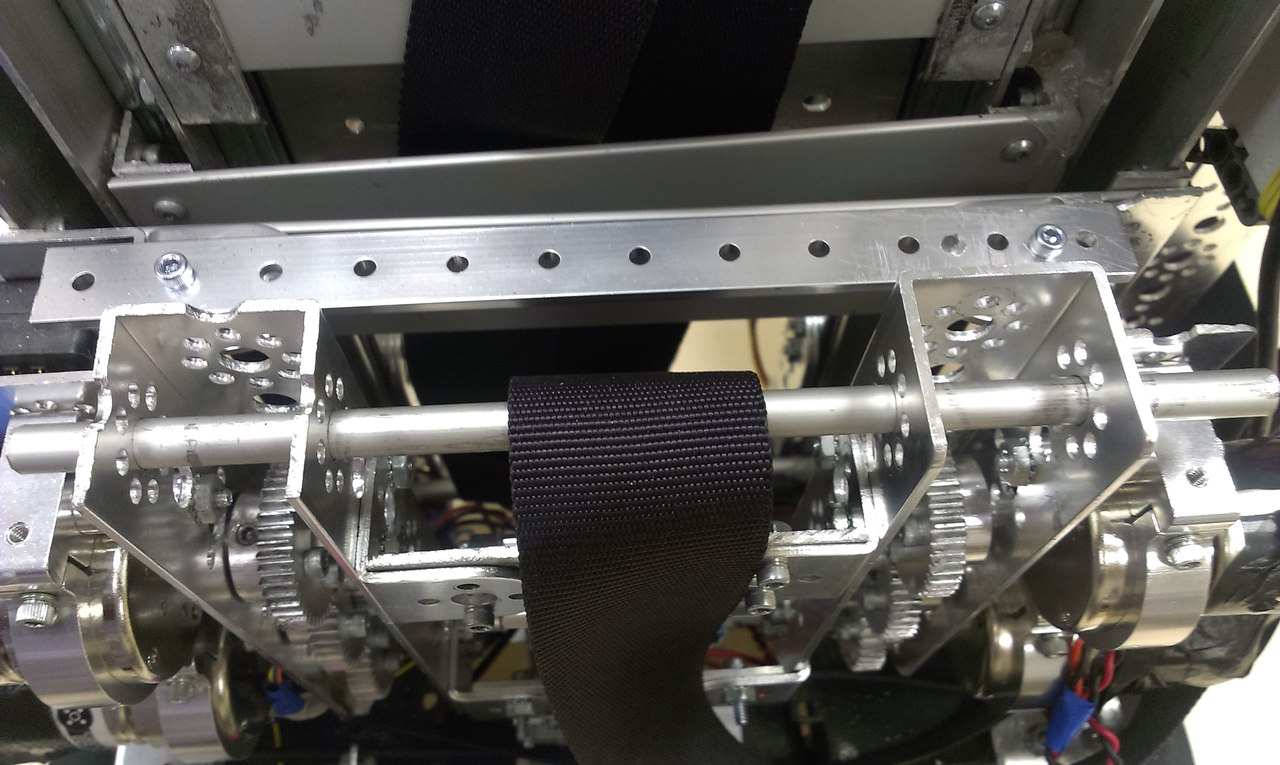
\includegraphics[scale=0.2]{days/06.12.14/images/02}}
	  		\caption{Rib of rigidity}
	  	\end{minipage}
	  \end{figure}
	  
    \end{enumerate}
    
	\item Results: 
	\begin{enumerate}
	  \item Drawing for bucket was created.
	  
	  \item Material for bucket was chosen.
	  
	  \item MEL was strengthened.
	  
    \end{enumerate}
    
	\item Tasks for the next meetings:
	\begin{enumerate}
	  \item To make a new bucket.
	  
    \end{enumerate}     
\end{enumerate}
\fillpage
